\documentclass[notheorems,serif]{beamer}

%选用主题
%\usetheme{Rochester}
%\usetheme{default}
%\usetheme{AnnArbor}
%\usetheme{Antibes}
%\usetheme{Bergen}
%\usetheme{Berkeley}
%\usetheme{Berlin}
%\usetheme{Boadilla}
%\usetheme{CambridgeUS}
%\usetheme{Copenhagen}
%\usetheme{Darmstadt}
%\usetheme{Dresden}
%\usetheme{Frankfurt}
%\usetheme{Goettingen}
%\usetheme{Hannover}
%\usetheme{Ilmenau}
%\usetheme{JuanLesPins}
%\usetheme{Luebeck}
\usetheme{Madrid}
%\usetheme{Malmoe}
%\usetheme{Marburg}
%\usetheme{Montpellier}
%\usetheme{PaloAlto}
%\usetheme{Pittsburgh}
%\usetheme{Rochester}
%\usetheme{Singapore}
%\usetheme{Szeged}
%\usetheme{Warsaw}

% As well as themes, the Beamer class has a number of color themes
% for any slide theme. Uncomment each of these in turn to see how it
% changes the colors of your current slide theme.

%\usecolortheme{albatross}
%\usecolortheme{beaver}
%\usecolortheme{beetle}
%\usecolortheme{crane}
%\usecolortheme{dolphin}
%\usecolortheme{dove}
%\usecolortheme{fly}
%\usecolortheme{lily}
%\usecolortheme{orchid}
%\usecolortheme{rose}
%\usecolortheme{seagull}
%\usecolortheme{seahorse}
%\usecolortheme{whale}
%\usecolortheme{wolverine}

%设置被cover的内容不显示
%\setbeamercovered{transparent}

\useinnertheme{rounded}
\usecolortheme{default}

%调用包
\usepackage[no-math, cm-default]{fontspec}
\usepackage{xltxtra}
\usepackage{xunicode}   
\usepackage{xcolor}
\usepackage{unicode-math} % 使用 unicode-math 设置数学字体
\usepackage{amsmath,amssymb}
\usepackage{xeCJK}
\usepackage{multimedia}
\usepackage{listings}
\usepackage{subfigure,caption}
%\usepackage{multicol}
\usepackage{multirow}


\renewcommand{\normalsize}{\wuhao}

%将系统字体名映射为逻辑字体名称,主要是为了维护的方便  
\newcommand\fnhei{Adobe 黑体 Std}  
\newcommand\fnsong{Adobe 宋体 Std}  
\newcommand\fnkai{Adobe 楷体 Std}  
\newcommand\fnmono{DejaVu Sans Mono}  
\newcommand\fnroman{Times New Roman}  

\renewcommand{\normalsize}{\wuhao}

%%设置常用中文字号,方便调用  
\newcommand{\erhao}{\fontsize{22pt}{\baselineskip}\selectfont}  
\newcommand{\xiaoerhao}{\fontsize{18pt}{\baselineskip}\selectfont}  
\newcommand{\sanhao}{\fontsize{16pt}{\baselineskip}\selectfont}  
\newcommand{\xiaosanhao}{\fontsize{15pt}{\baselineskip}\selectfont}  
\newcommand{\sihao}{\fontsize{14pt}{\baselineskip}\selectfont}  
\newcommand{\xiaosihao}{\fontsize{12pt}{\baselineskip}\selectfont}  
\newcommand{\wuhao}{\fontsize{10.5pt}{\baselineskip}\selectfont}  
\newcommand{\xiaowuhao}{\fontsize{9pt}{\baselineskip}\selectfont}  
\newcommand{\liuhao}{\fontsize{7.5pt}{\baselineskip}\selectfont}  
\newcommand{\bahao}{\fontsize{3.5pt}{\baselineskip}\selectfont}  

\setCJKmainfont[BoldFont=\fnhei]{\fnkai}  
\setCJKsansfont[BoldFont=\fnhei]{\fnkai}  
\setCJKmonofont{\fnkai}  

%楷体  
\newfontfamily\KAI {\fnkai}  
\newcommand{\kai}[1]{{\KAI#1}}  
%黑体  
\newfontfamily\HEI{\fnhei}  
\newcommand{\hei}[1]{{\HEI#1}}  


%%%%%%%%%%%%%%%%%%%% 设置数学公式的字体 %%%%%%%%%%%%%%%%%%%%%%%%%%%%%
%\setmathfont{Latin Modern Math}
%\usepackage{unicode-math}
%\setmainfont{TeX Gyre Termes} % 正文字体
\setmathfont{TeX Gyre Termes Math}
%%%%%%%%%%%%%%%%%%%%%%%%%%%%%%%%%%%%%%%%%%%%%%%%%%%%%%%%%%%%%%%%%%%%%

%英文  
\newfontfamily\ENF{\fnroman}  
\newcommand{\en}[1]{\,{\ENF#1}\,}


%连字符
\defaultfontfeatures{Mapping=tex-text}

%中文断行
\XeTeXlinebreaklocale "zh"
\XeTeXlinebreakskip = 0pt plus 1pt minus 0.1pt


%%%% 定理类环境的定义 %%%%
\newtheorem{example}{\hei{例子}} 
\newtheorem{problem}{\hei{问题}}           
\newtheorem{algorithm}{\hei{算法}}
\newtheorem{theorem}{\hei{定理}}
\newtheorem{definition}{\hei{定义}}
\newtheorem{axiom}{\hei{公理}}
\newtheorem{property}{\hei{性质}}
\newtheorem{proposition}{\hei{命题}}
\newtheorem{lemma}{\hei{引理}}
\newtheorem{corollary}{\hei{推论}}
\newtheorem{remark}{\hei{注解}}
\newtheorem{condition}{\hei{条件}}
\newtheorem{conclusion}{\hei{结论}}
\newtheorem{assumption}{\hei{假设}}

%重定义一些环境的名字
\renewcommand{\proofname}{\hei{证明}}
\renewcommand\tablename{\hei{表}}
\renewcommand\figurename{\hei{图}}

\newcommand{\marking}{\textcolor[rgb]{1.00,0.00,0.00}}
%选用主题
\usetheme{Madrid}

\usepackage[no-math, cm-default]{fontspec}
\usepackage{xltxtra}
\usepackage{xunicode}   
\usepackage{xcolor}
%\usepackage{unicode-math} % 使用 unicode-math 设置数学字体
\usepackage{amsmath, amssymb}
\usepackage{xeCJK}
\usepackage{multimedia}
\usepackage{listings}
\usepackage{caption}
\usepackage{multirow}
\usepackage{color, subcaption}
\usepackage{makecell}
\usepackage{algorithm}
\usepackage{algpseudocode}

%将系统字体名映射为逻辑字体名称,主要是为了维护的方便  
\newcommand\fnhei{Adobe 黑体 Std}  
\newcommand\fnsong{Adobe 宋体 Std}  
\newcommand\fnkai{Adobe 楷体 Std}  
\newcommand\fnmono{DejaVu Sans Mono}  
\newcommand\fnroman{Times New Roman}  

% 定理类环境的定义
\newtheorem{definition}{定义}[section]
\newtheorem{property}{性质}[section]
\newtheorem{lemma}{引理}[section]
\newtheorem{theorem}{定理}[section]
\newtheorem{corollary}{推论}[section]
\newtheorem{example}{算例}
\newtheorem{remark}{注}
\newtheorem{assumption}{假设}
\newtheorem{continue}{续}

\newcommand{\highlightit}{\textcolor[rgb]{1.00,0.00,0.00}}


%---SHORTCUTS--------------------------------------------------------------------------------------
\newcommand\xor{\mathbin{\char`\^}}
\DeclareMathOperator{\res}{Res}
\DeclareMathOperator{\sgn}{sgn}
\DeclareMathOperator{\supp}{supp}
\DeclareMathOperator{\as}{as}
\newcommand{\slant}[1]{\slshape #1\normalfont}
\newcommand{\dd}[2]{\frac{d#1}{d#2}} 
\newcommand{\ddx}{\frac{d}{dx}}
\newcommand{\ddt}{\frac{d}{dt}}
\newcommand{\dds}{\frac{d}{ds}}
\newcommand{\pd}[1]{\ds\frac{\partial}{\partial #1 }}
\newcommand{\pdd}[2]{\ds\frac{\partial #1}{\partial #2 }}
\newcommand{\mdd}[3]{\ds\frac{\partial^{#3} #1}{\partial #2^{#3} }}
\newcommand{\x}{\ _\Box}
\newcommand{\ds}{\displaystyle}
\newcommand{\Bold}{\noindent \bfseries}
\newcommand{\Norm}{\normalfont}
\newcommand{\exl}[1]{\textcolor{NavyBlue}{\Bold Exercise #1 \Norm}}
\newcommand{\ex}{\textcolor{NavyBlue}{\Bold Problem: \Norm}}
\newcommand{\sol}{\textcolor{Mulberry}{\Bold Solution: \Norm}}
\newcommand{\pf}{\textcolor{Mulberry}{\Bold Proof: \Norm}}
\newcommand{\Title}[1]{\LARGE\Bold \textcolor{Sepia}{#1}\Norm\normalsize \vspace{10pt} \newline}
\newcommand{\prop}{\Bold \textcolor{YellowOrange}{ Proposition:} \Norm}
\newcommand{\propl}[1]{\Bold \textcolor{YellowOrange}{ Proposition #1:} \Norm}
\newcommand{\rk}{\Bold \textcolor{YellowOrange}{ Remark:} \Norm}
\newcommand{\rmk}[1]{\Bold\textcolor{YellowOrange}{#1} \Norm}
\newcommand{\thm}[1]{\Bold \textcolor{YellowOrange}{ Theorem #1} \Norm}
\newcommand{\ind}{\indent\indent}

\newcommand{\red}{\color{red}}
\newcommand{\blue}{\color{blue}}

\newcommand{\mycomment}[1]{} % 默认不显示注释







\setbeamercovered{transparent}

\begin{document}

\title{无稳定化项的虚单元方法}
\author{陈春雨}
\institute[XTU]{
    \vspace{5pt}
    cbtxs@smail.xtu.edu.cn\\
\vspace{5pt}

合作者:黄学海(上海财经大学),魏华祎(湘潭大学)\\

湘潭大学\\
数学与计算科学学院
}
 
\date
{
    \today
}

\pgfdeclareimage[height=1cm]{institution-logo}{../figures/xtu.pdf}

\logo{\pgfuseimage{institution-logo}}

\frame[plain]{\titlepage}

\AtBeginSection[]{

  \frame<beamer>{ 

    \frametitle{Outline}   

    \tableofcontents[currentsection] 
  }
}
\section{虚单元方法简介}
%\begin{frame}
%    \frametitle{虚单元方法简介}
%\begin{minipage}[b]{0.55\linewidth}
%\end{minipage}
%\hfill
%\begin{minipage}[b]{0.4\linewidth}
%    \centering
%    \begin{figure}[htpb]
%        \centering
%        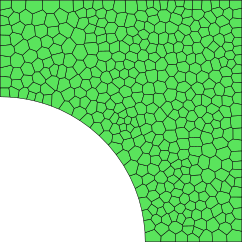
\includegraphics[width=0.5\textwidth]{../figures/voronoi_quad_circle.pdf}
%        \caption{多边形网格}
%    \end{figure}
%
%    \begin{figure}[htpb]
%        \centering
%        \includegraphics[width=0.6\textwidth]{../figures/polyhedron.png}
%        \caption{多面体网格}
%    \end{figure}
%\end{minipage}
%\end{frame}
\begin{frame}\frametitle{Poisson 方程}
\begin{minipage}[b]{0.6\linewidth}
考虑 $\Omega$ 上的 Poisson 方程问题:
$$
\left\{
\begin{aligned}
-\Delta u &= f \quad \text{in} \quad \Omega, \\
u &= 0 \quad \text{on} \quad \partial \Omega,
\end{aligned}
\right.
$$
其中 $f \in L^2(\Omega)$。其对应的变分问题为:寻找 $u \in H^1_0(\Omega)$,使得
$$
a(u, v) = (f, v) \quad \forall v \in H^1_0(\Omega),
$$
其中 
$$
a(u, v) = \int_{\Omega} \nabla u \cdot \nabla v \, \mathrm{d} x
$$
\end{minipage}
\hfill
\begin{minipage}[b]{0.38\linewidth}
    \centering
    \begin{figure}[htpb]
        \centering
        
\includegraphics[width=0.65\textwidth]{../figures/domain_quad.pdf}
        \caption{正方形区域 $\Omega$}
    \end{figure}
\end{minipage}

\end{frame}

\begin{frame}
\frametitle{Poisson 方程的线性有限元方法}
\begin{minipage}[b]{0.6\linewidth}
\vspace{10pt}
\begin{itemize}
\only<1>{
\item 将 $\Omega$ 三角剖分为 $\mathcal{T}_h$。
\item 定义局部有限元 $(V_k^K, K, \mathcal{N})$,
    其中 $V_k^K := \mathbb{P}_1(K)$。自由度 $\mathcal{N}$ 为顶点函数值:
    $$
    \mathcal{N}_i(v) = v(x_i)
    $$
    \begin{figure}[htpb]
        \centering
        \includegraphics[width=0.9\textwidth]{../figures/lambda.png}
        \caption{基函数}
    \end{figure}
}
\only<2>{
\item 建立全局有限元空间 $V_k$:
    $$
    V_k = \{v_h \in H^1(\Omega): v_h|_K \in V_k^K, \forall K \in
    \mathcal{T}_h\}.
    $$
\item 求解有限元问题:寻找 $u_h \in V_k$,使得
    $$
    a_h(u_h, v_h) = (f, v_h) \quad \forall v_h \in V_k,
    $$
    其中
    $$
    a_h(u_h, v_h) = \sum_{K \in \mathcal{T}_h} \int_K \nabla u_h \cdot \nabla v_h \,
    \mathrm{d} x
    $$
\vspace{15pt}
}
\end{itemize}
\end{minipage}
\hfill
\begin{minipage}[b]{0.38\linewidth}
    \begin{figure}[htpb]
        \centering
        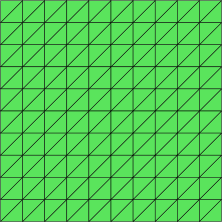
\includegraphics[width=0.5\textwidth]{../figures/struct_triangle_mesh.pdf}
        \caption{三角剖分}
    \end{figure}
    \begin{figure}[htpb]
        \centering
        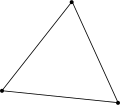
\includegraphics[width=0.4\textwidth]{../figures/triangle.pdf}
        \caption{三角形 $K$}
    \end{figure}
\vspace{10pt}
\end{minipage}
\end{frame}

\begin{frame}
    \frametitle{Poisson 方程的虚单元方法}
\begin{minipage}[b]{0.6\linewidth}
\begin{itemize}
\item 将 $\Omega$ 剖分为多边形网格 $\mathcal{T}_h$,
\item 定义局部虚单元 $(V_k^K, K, \mathcal{N})$,
    其中 
    $$
    V_k^K := \{v \in H^1(K): v|_{\partial K} \in \mathbb{P}_1(\partial K),
    \Delta v = 0\}.
    $$ 
    自由度 $\mathcal{N}$ 为顶点上的函数值。
    \begin{figure}[htpb]
        \centering
        \includegraphics[width=0.9\textwidth]{../figures/vemlambda.png}
        \caption{虚单元基函数}
    \end{figure}
    \uncover<2>{
    \vspace{-10pt}
    \centering{\marking{虚单元基函数是未知的!但是到 $\mathbb{P}_1(K)$
    的 $H^1$ 投影 $\Pi_h^K$ 是已知的。}}
    \vspace{10pt}
}
\end{itemize}
\end{minipage}
\hfill
\begin{minipage}[b]{0.38\linewidth}
    \centering
    \begin{figure}[htpb]
        \centering
        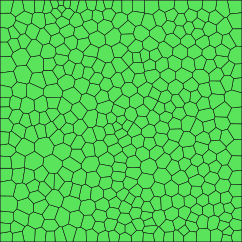
\includegraphics[width=0.6\textwidth]{../figures/voronoi_quad.pdf}
        \caption{多边形网格}
    \end{figure}
    \begin{figure}[htpb]
        \centering
        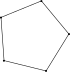
\includegraphics[width=0.5\textwidth]{../figures/polygon.pdf}
        \caption{多边形 $K$}
    \end{figure}
\end{minipage}
\end{frame}

\begin{frame}
    \frametitle{Poisson 方程的虚单元方法}
\begin{minipage}[b]{0.6\linewidth}
\begin{itemize}
\item 建立虚单元空间 $V_k$:
$$
V_k = \{v_h \in H^1(\Omega): v_h|_K \in V_k^K, \forall K \in
\mathcal{T}_h\}.
$$
\item 求解虚单元问题:寻找 $u_h \in V_k$,使得
$$
a_h(u_h, v_h) = (f, \Pi_hv_h) \quad \forall v_h \in V_k,
$$
离散双线性型 $a_h$ 定义如下:
$$
a_h(u_h, v_h) = \sum_{K \in \mathcal{T}_h} a_h^K(u_h, v_h) 
$$
\vspace{40pt}
\end{itemize}
\end{minipage}
\hfill
\begin{minipage}[b]{0.38\linewidth}
    \centering
    \begin{figure}[htpb]
        \centering
        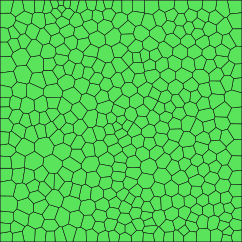
\includegraphics[width=0.6\textwidth]{../figures/voronoi_quad.pdf}
        \caption{多边形网格}
    \end{figure}
    \begin{figure}[htpb]
        \centering
        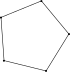
\includegraphics[width=0.5\textwidth]{../figures/polygon.pdf}
        \caption{多边形 $K$}
    \end{figure}
\end{minipage}
\end{frame}

\begin{frame}
    \frametitle{Poisson 方程的虚单元方法}
\begin{minipage}[b]{0.6\linewidth}
\begin{enumerate}
    \item[] 局部双线性型 $a_h^K$ 定义如下:
    $$
    \begin{aligned}
    a_h^K(u_h, v_h) = & \int_K \nabla \Pi_h^K u_h \cdot \nabla \Pi_h^K v_h \, \mathrm{d}
    x\\
    \uncover<2->{
    & \marking{+ S_h^K(u_h - \Pi_h^K u_h, v_h - \Pi_h^K v_h)}.
    }
    \end{aligned}
    $$
    \uncover<3->{
    其中 $S_h^K$ 是一个稳定化项,需要满足:
    $$
    C_* |v|_{1} \leq S_h^K(v, v) \leq C^*
    |v|_{1} 
    $$
    对于任意的 $v \in \ker{\Pi_h^K} \cap V_k^K$ 成立。
    }
\end{enumerate}
\vspace{40pt}
\end{minipage}
\hfill
\begin{minipage}[b]{0.38\linewidth}
    \centering
    \begin{figure}[htpb]
        \centering
        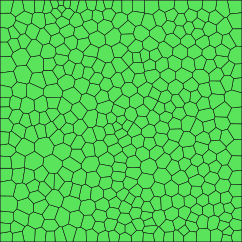
\includegraphics[width=0.6\textwidth]{../figures/voronoi_quad.pdf}
        \caption{多边形网格}
    \end{figure}
    \begin{figure}[htpb]
        \centering
        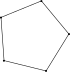
\includegraphics[width=0.5\textwidth]{../figures/polygon.pdf}
        \caption{多边形 $K$}
    \end{figure}
\end{minipage}
\end{frame}

\begin{frame}
    \frametitle{虚单元方法的优缺点}
\begin{minipage}[b]{0.6\linewidth}
\textbf{优点:}
\begin{itemize}
    \item \textbf{网格要求低}:可以在任意多边形网格上计算。
    \item \textbf{方便定义高正则性空间}:可以定义 $H^m$
        协调非协调空间,且多项式次数只需要 $k \geq m$。
\end{itemize}
\vspace{10pt}
\textbf{缺点:}
\begin{itemize}
    \item \textbf{实现复杂}:相比于有限元,虚单元实现更为复杂。 
    \item \textbf{稳定化项}:在非线性问题中,系数的选取对数值结果有较大影响。
\end{itemize}
\end{minipage}
\hfill
\begin{minipage}[b]{0.38\linewidth}
    \centering
    \begin{figure}[htpb]
        \centering
        \includegraphics[width=0.65\textwidth]{../figures/four.jpg}
        \caption{四叉树网格}
    \end{figure}
\end{minipage}
\end{frame}

\begin{frame}
    \frametitle{去除稳定化项}
    \begin{minipage}[b]{0.55\linewidth}
    对于任意多边形多面体 $K$,找到一个空间 $\mathbb{V}(K)$,以及一个到
    $\mathbb{V}(K)$ 的投影算子 $Q^K$,满足:
    \begin{itemize}
        \item 对于任意 $v \in V_k^K$, $Q^K \nabla v$ 可以基于 $v$
            的自由度进行计算。
        \item $\mathbb{V}(K)$ 要足够大,以至于满足如下范数等价关系:
            $$
            \|Q^K \nabla v\| \eqsim \|\nabla v\| \quad \forall v \in V_k^K.
            $$
    \end{itemize}
\end{minipage}
\hfill
\begin{minipage}[b]{0.44\linewidth}
    \begin{figure}[htpb]
        \centering
        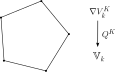
\includegraphics[width=0.8\textwidth]{../figures/projection.pdf}
        \caption{投影算子 $Q^K$}
    \end{figure}
\end{minipage}
\end{frame}

\section{$H(\mathrm{div})$ 协调宏元空间}
\begin{frame}
  \frametitle{网格条件}
  网格 $\mathcal{T}_h$ 要求满足如下条件:
  \begin{itemize}
    \item 对于任意的单元 $K \in \mathcal{T}_h$ 以及面 $F \in \mathcal{F}_h^r$,
        $1 \leq r \leq d-1$ 关于一个半径为 $\rho_K$ 的球是 star-shaped 的,且
        $\rho_K/h_K$ 有下界。
    \item 任意单元 $K \in \mathcal{T}_h$ 存在一个拟一致的的单纯形网格
        $\mathcal{T}_K$ 剖分 $K$,且 $\cup_{K \in \mathcal{T}_h}\mathcal{T}_K$
        是一个形状正则的单纯形网格。
  \end{itemize}
  \vspace{10pt}
\begin{minipage}[b]{0.49\linewidth}
    \begin{figure}[htpb]
      \centering
      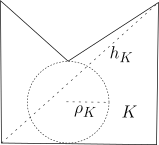
\includegraphics[width=0.55\textwidth]{../figures/star-shaped.pdf}
      \caption{star-shaped}
    \end{figure}
\end{minipage}
\hfill
\begin{minipage}[b]{0.49\linewidth}
    \centering
    \begin{figure}[htpb]
        \centering
        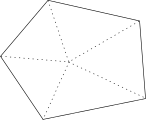
\includegraphics[width=0.55\textwidth]{../figures/splite_polygon.pdf}
        \caption{拟一致单纯形网格}
    \end{figure}
\end{minipage}

\end{frame}

\begin{frame}
    \frametitle{有限元微分 $d-2$ 形式}
对于 $T \in \mathcal{T}_K$,以 $\mathbb{P}_k(T, \mathbb{K})$
为形函数空间,定义如下自由度:
$$
\begin{aligned}
((\bsn_{1}^{e})^{\mathsf{T}}\tau\bsn_{2}^{e},q)_{e}, & \quad q\in\mathbb{P}_{k}(e),e\in\mathcal{E}(T), \\
(\mathrm{div}_{F}(\tau\bsn),q)_{F}, & \quad q\in\mathbb{P}_{k-1}(F)/\mathbb{R},F\in\mathcal{F}(T), \\
(\tau\bsn,\bsq)_F, & \quad q\in\mathbb{P}_{k-2}(F;\mathbb{K})\bsx,F\in\mathcal{F}(T), \\
(\operatorname{div}\tau,q)_{T}, & \quad q\in\mathbb{P}_{k-3}(T;\mathbb{K})\bsx, \\
(\tau,q)_{T}, & \quad \bsq\in\mathbb{P}_{k-2}(T;\mathbb{K})\cap\ker(\bsx).
\end{aligned}
$$
定义 $d-2$ 形式空间 $V^{d-2}_k$:
$$
\begin{aligned}
V^{d-2}_k = \{\tau \in L^2(K; \mathbb{K}) : & \tau|_T \in \mathbb{P}_k(T, \mathbb{K}),
\forall T \in \mathcal{T}_K, \\
& \text{ first three conditions are single-valued}\}.
\end{aligned}
$$
\uncover<2->{
\small{
\marking{
$d = 2$ 时 $V^{d-2}_k$ 为 Lagrange 元空间。
$d = 3$ 时 $V^{d-2}_k$ 为 Ned\'el\'ec 元空间。
}
}
}
\end{frame}

\begin{frame}
    \frametitle{$H(div)$ 协调有限元空间: BDM 元}
    对于 $k\geq2$,定义 $H(\mathrm{div})$ BDM 元空间 $V^{BDM}_{k-1}$:
    $$
    V^{BDM}_{k-1}(K) := \{\bsv \in H(\diver, K) : \bsv|_T \in
    \mathbb{P}_{k-1}(T; \mathbb{R}^d), \forall T \in \mathcal{T}_K\}.
    $$
    BDM 元在单纯形 $T$ 上的局部自由度为:
    $$
    \begin{aligned}
        (v\cdot\bsn,q)_{F}, & \quad
        q\in\mathbb{P}_{k-1}(F),F\in\mathcal{F}(T), \\
        (\diver v, q)_{T}, & \quad q\in\mathbb{P}_{k-2}(T)/\mathbb{R}\\
        (v, \bsq)_T, & \quad
        \bsq\in\mathbb{P}_{k-3}(T;\mathbb{K})\bsx.
    \end{aligned}
    $$
    定义 $V^{BDM}_{k-1}$ 的迹零子空间:
    $$
    \mathring{V}_{k-1}^{\mathrm{BDM}}(K):=V_{k-1}^{\mathrm{BDM}}(K)\cap\bsH_{0}(\mathrm{div},K).
    $$
\end{frame}

\begin{frame}
    \frametitle{$H(\mathrm{div})$ 协调有限元空间: RT 元}
    对于 $k=1$ 的情况,定义最低阶 RT 元空间 $V^{RT}$:
    $$
    V^{RT}(K) := \{\bsv \in H(\diver, K) : \bsv|_T \in
        \mathbb{P}_{0}(T; \mathbb{R}^d) + \bsx\mathbb{P}_{0}(T),
    \forall T \in \mathcal{T}_K\}.
    $$
    RT 元在单纯形 $T$ 上的局部自由度为:
    $$
    (v\cdot\bsn,q)_{F}, \quad
    q\in\mathbb{P}_{0}(F),F\in\mathcal{F}(T)
    $$
    定义其迹零子空间:
    $$
    \mathring{V}^{\mathrm{RT}}(K):=V^{\mathrm{RT}}(K)\cap\bsH_{0}(\mathrm{div},K).
    $$
\end{frame}

\begin{frame}
    \frametitle{有限元复形}
    对于 $k\geq2$ 的情况,如下有限元复形是恰当的:
    $$
    \begin{aligned}
        V_{k}^{d-2}(K) & \xrightarrow{\mathrm{div~skw}}
        V_{k-1}^{\mathrm{BDM}}(K) \xrightarrow{\mathrm{div}} V_{k-2}^{L^{2}}(K)
        \to 0,\\
        V_{1}^{d-2}(K) & \xrightarrow{\mathrm{div~skw}}
        V^{\mathrm{RT}}(K) \xrightarrow{\mathrm{div}} V_{0}^{L^{2}}(K)
        \to 0,\\
        \mathring{V}_{k}^{d-2}(K) & \xrightarrow{\mathrm{div~skw}}
        \mathring{V}_{k-1}^{\mathrm{BDM}}(K) \xrightarrow{\mathrm{div}}
        \mathring{V}_{k-2}^{L^{2}}(K) \to 0,\\
        \mathring{V}_{1}^{d-2}(K) & \xrightarrow{\mathrm{div~skw}}
        \mathring{V}^{\mathrm{RT}}(K) \xrightarrow{\mathrm{div}}
        \mathring{V}_{0}^{L^{2}}(K) \to 0,
    \end{aligned}
    $$
    其中 $\mathring{V}_{k-2}^{L^{2}}(K) = V_{k-2}^{L^{2}}(K) / \mathbb{R}$。
    $$
    V_{k-2}^{L^{2}}(K) = \{\tau \in L^2(K; \mathbb{K}) : \tau|_T \in
    \mathbb{P}_{k-2}(T), \forall T \in \mathcal{T}_K\}.
    $$
\end{frame}

\begin{frame}
    \frametitle{$H(\mathrm{div})$ 协调宏元空间 $V^{\mathrm{div}}_{k-1}$}
    定义 $H(\mathrm{div})$ 协调宏元空间 $V^{\mathrm{div}}_{k-1}$(K):
    $$
    V^{\mathrm{div}}_{k-1}(K) := \{\bsv \in V^{BDM}_{k-1}(K) : \diver
    \bsv \in \mathbb{P}_{k-2}(K)\}.
    $$
    对于 $k=1$ 的情况,定义:
    $$
    V^{\mathrm{div}}_{0}(K) := \{\bsv \in V^{RT}(K) : \diver
    \bsv \in \mathbb{P}_{0}(K)\}.
    $$
    根据有限元复形,可以对 $V^{\mathrm{div}}_{k-1}(K)$ 做如下分解:
    $$
    V^{\mathrm{div}}_{k-1}(K) = \mathrm{div~skw}V_{k}^{d-2}(K) \oplus 
    (\boldsymbol{x-x}_K)\mathbb{P}_{\max\{k-2, 0\}}(K).
    $$
    如下复形是恰当的:
    $$
    \begin{aligned}
        V_{k}^{d-2}(K) & \xrightarrow{\mathrm{div~skw}}
        V^{\mathrm{div}}_{k-1}(K) \xrightarrow{\mathrm{div}}
        (\boldsymbol{x-x}_K)\mathbb{P}_{\max\{k-2, 0\}}(K) \to 0
    \end{aligned}
    $$
\end{frame}

\begin{frame}
    \frametitle{$H(\mathrm{div})$ 协调宏元空间 $\mathbb{V}^{\mathrm{div}}_{k-1}$}
    $V^{\mathrm{div}}_{k-1}$ 在 $K$ 的边界上不是多项式,所以取其一个子空间 
    $\mathbb{V}^{\mathrm{div}}_{k-1}$:
    $$
    \mathbb{V}^{\mathrm{div}}_{k-1}(K) := \{\bsv \in
        V^{\mathrm{div}}_{k-1}(K) :
        \bsv \cdot \bsn|_F \in \mathbb{P}_{k-1}(F),
    \forall F \in \mathcal{F}(K)\}.
    $$
    其自由度为:
    $$
    \begin{aligned}
        (v\cdot\bsn,q)_{F}, & \quad
        q\in\mathbb{P}_{k-1}(F),F\in\mathcal{F}(K), \\
        (\diver v, q)_{K}, & \quad q\in\mathbb{P}_{\max\{k-2, 0\}}(K)/\mathbb{R}, \\
        (v, \bsq)_K, & \quad
        \bsq\in \diver \mathring{V}_k^{d-2}(K).
    \end{aligned}
    $$
    $\mathbb{V}_{k-1}^{div}$ 中的函数有以下范数等价性:
    $$
    \|\bsv\|_{0, K} \eqsim h_K\|\diver \bsv\|_{0, K} + 
    \sup_{\psi \in \diver \mathring{V}_k^{d-2}(K)}\frac{(\bsv,
    \psi)_K}{\|\psi\|_{0, K}} + \sum_{F \in \mathcal{F}(K)}h_F^{1/2}\|v\cdot
    \bsn\|_{0, F}.
    $$
\end{frame}

\section{无稳定子虚单元方法}
\begin{frame}
\frametitle{非协调虚单元方法:空间}
定义非协调虚单元空间:
$$
\begin{aligned}
    V_k(K) := \{v \in H^1(K): & \partial_n v|_{F} \in \mathbb{P}_{k-1}(F), 
        \forall F \in \mathcal{F}(K), \
    \Delta v \in \mathbb{P}_{k}(K),\\
    & (v-\Pi_k^K v, q)_K = 0 \quad \forall q \in
    \mathbb{P}_{k-2}^{\perp}(K)\}.
\end{aligned}
$$
其中 $\Pi_k^K$ 是到 $\mathbb{P}_k(K)$ 的 $H^1$ 投影。
虚单元自由度为:
$$
\begin{aligned}
    \frac{1}{|F|}(v, q)_{F}, & \quad q \in \mathcal{M}_{k-1}(F), \\
    \frac{1}{|K|}(v, q)_{K}, & \quad q\in \mathcal{M}_{k-2}(K), \\
\end{aligned}
$$
其中 $\mathcal{M}_{k-1}(F)$ 和 $\mathcal{M}_{k-2}(K)$ 分别为 $F$ 和 $K$
上的缩放单项式。
定义 $Q_{K, k-1}^{\mathrm{div}}$ 为 $\nabla V_k(K)$ 到
$\mathbb{V}^{\mathrm{div}}_{k-1}(K)$ 的 $L^2$ 投影。
$$
(Q_{K, k-1}^{\mathrm{div}}\nabla v, \bsw)_K := (\nabla v,
\bsw)_K = -(v, \diver \bsw)_K + \langle v, \bsw 
\cdot \bsn\rangle_{\partial K}.
$$
\end{frame}

\begin{frame}
    \frametitle{非协调虚单元方法:范数等价性}
    \begin{lemma}
        成立如下 Inf-Sup 条件:
        $$
        \|\nabla v\| \leq C \sup_{\bsw \in
        \mathbb{V}^{\mathrm{div}}_{k-1}(K)}\frac{(\nabla v,
        w)_K}{\|\bsw\|} \quad \forall v \in V_k(K).
        $$
        其中 $C$ 与网格尺寸无关,与多项式次数 $k$,空间维数 $d$, 多面体的
        star-shaped 参数,网格的拟一致性和形状正则性参数有关。
        
        如下范数等价性成立:
        $$
        \|Q_{K, k-1}^{\mathrm{div}}\nabla v\|_{0, K} \eqsim \|\nabla v\|_{0, K} 
        \quad \forall v \in V_k(K).
        $$
    \end{lemma}
\end{frame}

\begin{frame}
    \frametitle{Poisson 方程的无稳定子 $H^1$ 非协调虚单元方法}
无稳定子虚单元方法定义为:寻找 $u_h \in V_k$,使得
$$
a_h(u_h, v_h) = (f, Q_h v_h) \quad \forall v_h \in V_k,
$$
其中 $a_h$ 定义为:
$$
a_h(u_h, v_h) = \sum_{K \in \mathcal{T}_h} a_h^K(u_h, v_h),
$$
$$
a_h^K(u_h, v_h) = (Q_{K, k-1}^{\mathrm{div}}\nabla u_h, Q_{K,
k-1}^{\mathrm{div}}\nabla v_h)_K.
$$
单元离散双线性型 $a_h^K$ 满足如下稳定性条件:
$$
c_* |v|_{1, K}^2 \leq a_h^K(v, v) \leq C_* |v|_{1, K}^2 \quad \forall v \in
V_k^K.
$$
\begin{theorem}
假设 $u \in H^{k+1}(\Omega), f \in H^{k-1}(\Omega)$,则上述无稳定子虚单元方法
是稳定的,且有:
$$
|u - u_h|_{1, \Omega} \leq C h^{k}
(|u|_{k+1, \Omega} + |f|_{k-1, \Omega}).
$$
\end{theorem}
\end{frame}

\begin{frame}
\frametitle{协调虚单元方法:空间}
假设多面体的所有面都是单纯形,
定义 $H^1$ 协调虚单元空间:
$$
\begin{aligned}
    V_k(K) := \{v \in H^1(K): & v|_{\partial K} \in H^1(\partial K), v|_F \in 
        \mathbb{P}_k(e), \forall e \in \mathcal{F}(K),
    \Delta v \in \mathbb{P}_{k}(K),\\
    & (v-\Pi_k^K v, q)_K = 0 \quad \forall q \in
    \mathbb{P}_{k-2}^{\perp}(K)\}.
\end{aligned}
$$
其中 $\Pi_k^K$ 是到 $\mathbb{P}_k(K)$ 的 $H^1$ 投影。
虚单元自由度为:
$$
\begin{aligned} 
    v(\delta), & \quad \delta \in \mathcal{\Delta}_0(K), \\
    \frac{1}{|e|}(v, q)_{e}, & \quad q \in \mathcal{M}_{k-j-1}(e), \forall e \in
    \Delta_j(K), j = 1, \dots, d-1\\
    \frac{1}{|K|}(v, q)_{K}, & \quad q\in \mathcal{M}_{k-2}(K), \\
\end{aligned}
$$
其中 $\mathcal{M}_{k-j-1}(e)$ 和 $\mathcal{M}_{k-2}(K)$ 分别为 $e$ 和 $K$
上的缩放单项式。
定义 $Q_{K, k-1}^{\mathrm{div}}$ 为 $\nabla V_k(K)$ 到
$\mathbb{V}^{\mathrm{div}}_{k}(K)$ 的 $L^2$ 投影。
$$
(Q_{K, k}^{\mathrm{div}}\nabla v, \bsw)_K := (\nabla v,
\bsw)_K = -(v, \diver \bsw)_K + \langle v, \bsw 
\cdot \bsn\rangle_{\partial K}.
$$
\end{frame}

\begin{frame}
    \frametitle{协调虚单元方法:范数等价性}
    \begin{lemma}
        成立如下 Inf-Sup 条件:
        $$
        \|\nabla v\| \leq C \sup_{\bsw \in
        \mathbb{V}^{\mathrm{div}}_{k}(K)}\frac{(\nabla v,
        w)_K}{\|\bsw\|} \quad \forall v \in V_k(K).
        $$
        其中 $C$ 与网格尺寸无关,与多项式次数 $k$,空间维数 $d$, 多面体的
        star-shaep 参数,网格的拟一致性和形状正则性参数有关。
        
        如下范数等价性成立:
        $$
        \|Q_{K, k}^{\mathrm{div}}\nabla v\|_{0, K} \eqsim \|\nabla v\|_{0, K} 
        \quad \forall v \in V_k(K).
        $$
    \end{lemma}
\end{frame}

\begin{frame}
    \frametitle{Poisson 方程的无稳定子 $H^1$ 协调虚单元方法}
无稳定子虚单元方法定义为:寻找 $u_h \in V_k$,使得
$$
a_h(u_h, v_h) = (f, Q_h v_h) \quad \forall v_h \in V_k,
$$
其中 $a_h$ 定义为:
$$
a_h(u_h, v_h) = \sum_{K \in \mathcal{T}_h} a_h^K(u_h, v_h),
$$
$$
a_h^K(u_h, v_h) = (Q_{K, k}^{\mathrm{div}}\nabla u_h, Q_{K,
k}^{\mathrm{div}}\nabla v_h)_K.
$$
单元离散双线性型 $a_h^K$ 满足如下稳定性条件:
$$
c_* |v|_{1, K}^2 \leq a_h^K(v, v) \leq C_* |v|_{1, K}^2 \quad \forall v \in
V_k^K.
$$
\begin{theorem}
假设 $u \in H^{k+1}(\Omega), f \in H^{k-1}(\Omega)$,则上述无稳定子虚单元方法
是稳定的,且有:
$$
|u - u_h|_{1, \Omega} \leq C h^{k}
(|u|_{k+1, \Omega} + |f|_{k-1, \Omega}).
$$
\end{theorem}
\end{frame}

\begin{frame}
    \frametitle{程序实现:$\mathbb{V}^{\mathrm{div}}_{k-1}$ 的一组基函数}
    \begin{minipage}[b]{0.6\linewidth}
    在程序实现中,需要有一组 $\mathbb{V}^{\mathrm{div}}_{k-1}$
    的基函数,一方面用来计算 $Q_{K, k-1}^{\mathrm{div}}$
    的矩阵表示,另一方面为了投影后的结果可计算。

    \textbf{在二维情况}
    $\mathbb{V}^{\mathrm{div}}_{k-1}$ 可以分解为
    $$
    \mathbf{rot} V^{Lag}_k \oplus (\mathbf{x-x}_K)\mathbb{P}_{k-2}(K). 
    $$
    那么可以定义如下基函数:
    $$
    \mathbf{rot} \{\Phi^{Lag}_k/\phi_0\} \oplus (\mathbf{x-x}_K)
    \mathcal{M}_{k-2}(K).
    $$
    其中 $\Phi^{Lag}_k$ 是 Lagrange 元空间的基函数,$\phi_0$
    是中心点对应的基函数。
\end{minipage}
\hfill
\begin{minipage}[b]{0.38\linewidth}
    \centering
    \begin{figure}[htpb]
        \centering
        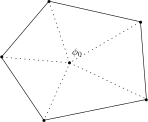
\includegraphics[width=0.8\textwidth]{../figures/lagrange_phi0.pdf}
        \caption{Lagrange 元中心点基函数}
    \end{figure}
\vspace{30pt}
\end{minipage}
\end{frame}

\section{数值结果}
\begin{frame}
\frametitle{数值算例:二阶椭圆方程}
考虑如下二阶椭圆方程:
$$
\left\{
\begin{aligned}
    -\Delta u + 2u & = f \quad \Omega\\
    u & = 0 \quad \partial\Omega
\end{aligned}
\right.
$$
其中 $\Omega = (0, 1)\times(0, 1)$,右端项和真解为:
$$
u = \sin(\pi x)\sin(\pi y), \quad f = (2\pi^2+2)\sin(\pi x)\sin(\pi y).
$$

\begin{figure}[htb p]
\centering
\begin{minipage}[t]{0.49\linewidth}
\centering
\includegraphics[width=4cm]{../figures/convex.pdf}
\captionsetup{font={small}}
\caption{凸多边形网格 $\mathcal T_0$}
\end{minipage}%
\begin{minipage}[t]{0.49\linewidth}
\centering
\includegraphics[width=4cm]{../figures/nonconvex.pdf}
\captionsetup{font={small}}
\caption{非凸多边形网格 $\mathcal T_1$}
\end{minipage}%
\centering
\end{figure}
\end{frame}

\begin{frame}
    \frametitle{数值结果:收敛性}
选择 $k = 1, 2, 5$ 在 SFNCVEM 和 SFCVEM 中进行计算。
以下是 SFNCVEM 在网格 $\mathcal T_0$ 和 $\mathcal T_1$ 上的数值结果。
可以看到 $\|u - Q_h u_h\|_0=O(h^{k+1})$ 和 $\|\nabla u -
Q_{h}\nabla_h u_h\|_0=O(h^{k})$, 
\begin{figure}[htbp]
\centering
\begin{minipage}[t]{0.49\linewidth}
\centering
\includegraphics[width=5.5cm]{../figures/stabfree/ncvem_convex.pdf}
%\caption{使用 $\mathcal T_0$ 的数值结果。}
\end{minipage}%
\begin{minipage}[t]{0.49\linewidth}
\centering
\includegraphics[width=5.5cm]{../figures/stabfree/ncvem_nonconvex.pdf}
%\caption{[使用 $\mathcal T_1$ 的数值结果。]}
\end{minipage}%
\centering
\caption{在网格 $\mathcal T_0$(左) 和 $\mathcal T_1$(右) 上,使用 $k=1, 2, 5$
的非协调 VEM 的误差 $\|u - Q_h u_h\|_0$ 和 $\|\nabla u - Q_{h}\nabla_h u_h\|_0$。}
\label{fig:rate1}
\end{figure}
\end{frame}

\begin{frame}
\frametitle{数值结果:收敛性}
以下是 SFCVEM 的数值结果。
同样,$\|u - Q_h u_h\|_0=O(h^{k+1})$ 和 $\|\nabla u - Q_{h}\nabla
u_h\|_0=O(h^{k})$。 

\begin{figure}[htbp]
\centering
\begin{minipage}[t]{0.49\linewidth}
\centering
\includegraphics[width=5.5cm]{../figures/stabfree/cvem_convex.pdf}
%\caption{使用 $\mathcal T_0$ 的数值结果。}
\end{minipage}%
\begin{minipage}[t]{0.49\linewidth}
\centering
\includegraphics[width=5.5cm]{../figures/stabfree/cvem_nonconvex.pdf}
%\caption{[使用 $\mathcal T_1$ 的数值结果。]}
\end{minipage}%
\centering
\caption{在网格 $\mathcal T_0$(左) 和 $\mathcal T_1$(右) 上,使用 $k=1, 2, 5$
的协调 VEM 的误差 $\|u - Q_h u_h\|_0$ 和 $\|\nabla u - Q_{h}\nabla u_h\|_0$。}
\label{fig:rate2}
\end{figure}
\end{frame}

\begin{frame}
    \frametitle{数值结果:零特征值与条件数}
构造如下三种不同的六边形,并计算四种虚单元方法在 $k=3$ 时的局部刚度矩阵的特征值。 
\begin{figure}[htbp]
\subfigure[规则六边形.]{
\begin{minipage}[t]{0.3\linewidth}
\centering
\includegraphics[width=1in]{../figures/stabfree/hexagon0.pdf}
\end{minipage}}%% 
\;\;% \quad
\subfigure[通过对规则六边形进行小扰动生成的准规则六边形.]
{\begin{minipage}[t]{0.3\linewidth}
\centering
\includegraphics[width=1in]{../figures/stabfree/hexagon1.pdf}
\end{minipage}}
\;\;% \quad
\subfigure[具有两个悬点的方形.]
{\begin{minipage}[t]{0.3\linewidth}
\centering
\includegraphics[width=0.9in]{../figures/stabfree/hexagon2.pdf}
\end{minipage}}
\caption{规则六边形(左),通过对规则六边形进行小扰动生成的准规则六边形(中),以及具有两个悬点的方形(右)。}
\end{figure} 
\end{frame}

\begin{frame}
    \frametitle{数值结果:零特征值与条件数}
不同六边形上局部刚度矩阵的最小非零特征值、最大特征值和条件数。
从中可以看出,这些量对于四种虚单元方法是相似的。
\only<1>{
\begin{table}[htbp] 
\centering
\caption{在规则六边形上,特征值和条件数的比较。}
\begin{tabular}{c|ccc}
\hline
\textbf{方法} & \textbf{最大特征值} & \textbf{最小特征值} & \textbf{条件数} \\ \hline
NCVEM & 975.5693189 & 0.309674737 & 3150.303211 \\ \hline
CVEM & 1012.488116 & 0.297206358 & 3406.683909 \\ \hline
SFNCVEM & 992.5956147 & 0.318932029 & 3112.248147 \\ \hline
SFCVEM & 1011.173331 & 0.298509692 & 3387.405362 \\
\hline
\end{tabular}
\end{table}
}
\only<2>{
\begin{table}[htbp]
\centering
\caption{在准规则六边形上,特征值和条件数的比较。}
\begin{tabular}{c|ccc}
\hline
\textbf{方法} & \textbf{最大特征值} & \textbf{最小特征值} & \textbf{条件数} \\ \hline
NCVEM   & 935.2883848 & 0.279027715 & 3351.955143 \\ \hline
CVEM    & 1014.672395 & 0.257370621 & 3942.456177 \\ \hline
SFNCVEM & 997.4831245 & 0.282126359 & 3535.589964 \\ \hline
SFCVEM  & 1047.876056 & 0.258970708 &
4046.311124 \\
\hline
\end{tabular}
\end{table}
}
\only<3>{
\begin{table}[htbp]
\centering
\caption{在具有两个悬点的方形上,特征值和条件数的比较。}
\begin{tabular}{c|ccc}
\hline
\textbf{方法} & \textbf{最大特征值} & \textbf{最小特征值} & \textbf{条件数} \\ \hline
 NCVEM   & 941.8571938&	0.21069027	&4470.340249 \\ \hline
 CVEM    & 1046.755495&	0.200435123	&5222.4155 \\ \hline
 SFNCVEM & 986.5963357&	0.212761106	&4637.108513 \\ \hline
 SFCVEM  & 1061.651989&	0.202074633	&5253.761808 \\
\hline
\end{tabular}
\end{table}
}
\end{frame}

\begin{frame}
\frametitle{数值结果:计算时间}

我们在凸多边形网格上进行实验。下面的表格展示了NCVEM、CVEM和SFNCVEM的组装时间相似。然而,由于SFCVEM需要将投影映射到一个高一个阶数的多项式空间,因此其计算时间较长。
\only<1>{
\begin{table}[htbp]
\centering
\caption{不同$k$值下四种VEM组装刚度矩阵所消耗的时间($h = 0.2$)。}
\begin{tabular}{c|cccc}
\hline
\textbf{k} & \textbf{2} & \textbf{4} & \textbf{8} & \textbf{10} \\ \hline
SFCVEM & 0.053684235 & 0.144996881 & 1.468627453 & 2.603836536 \\ \hline
SFNCVEM & 0.022516727 & 0.065697193 & 0.806378841 & 1.554260015 \\ \hline
CVEM & 0.021185875 & 0.059809923 & 0.600241184 & 1.160929918 \\ \hline
NCVEM & 0.0213027 & 0.061014891 & 0.596506596 & 1.129639149 \\
\hline
\end{tabular}
\end{table}
}
\only<2>{
\begin{table}[htbp]
\centering
\caption{不同$h$值下,$k=5$时四种VEM组装刚度矩阵所消耗的时间。}
\begin{tabular}{c|cccc}
\hline
\textbf{h} & \textbf{1} & \textbf{0.25} & \textbf{0.0625} & \textbf{0.03125} \\ \hline
SFCVEM & 0.039689541 & 0.199015379 & 1.74412179 & 4.75462532 \\ \hline
SFNCVEM & 0.018287182 & 0.100006819 & 0.81251812 & 2.465409517 \\ \hline
CVEM & 0.018686771 & 0.087426662 & 0.781031132 & 1.983617783 \\ \hline
NCVEM & 0.018309593 & 0.096345425 & 0.767129898 & 2.159288645 \\
\hline
\end{tabular}
\end{table}
}
\end{frame}

\begin{frame}
    \frametitle{\small{FEALPy:新一代简单、易用、高效、智能的 CAE 仿真计算引擎}}
\begin{figure}[htbp]
    \centering
    \includegraphics[width=1\linewidth]{../figures/fealpy.png}
\end{figure}

\end{frame}

\begin{frame}
\begin{figure}[htbp]
\centering
\includegraphics[width=1\textwidth]{../figures/suanhai.png}
\end{figure}
\end{frame}


\end{document}

